\section{Implementation}\label{implementation}

The following sections describe the implementation of the workflow system.
First of all the integration of WS-PGRADE/gUSE with the existing cloud architecture is described, followed by the configuration and trouble shooting of the system.
The last section explains different approaches to create workflows built on top of a sample application.

\subsection{Architecture}\label{architecture}

The existing QM-ROCT server infrastructure consists of various system components (see figure~\ref{fig:architecture}), which are loosely coupled as web services.
A server machine running an instance of XNAT can be accessed via the internet, so that researcher are able to upload and manage data using the graphical web interface.
The rest of the architecture is encapsulated in a private network.
Especially the OpenStack cloud is not reachable from the internet. The only accesspoint for XNAT, to send data processing jobs to the cloud, is a gateway server running a REST web-service.
The gateway server is responsible for communicating with the cloud control server to start a Virtual Machine, submit the incoming job and stop the VM again, when the processing is done.
When submitting a job from XNAT, using the XNAT pipeline system (see section~\ref{xnat}), no data files are transferred to the gateway server.
Only parameters are transferred, which are used to download the files via the XNAT Rest API.
the download happens inside the VM, which connects to XNAT for downloading data and for uploading the results.
This ensures, that no unnecessary file transfers are performed. 

When introducing gUSE to this infrastructure it is important to deploy it inside the private network, because the DCI bridge communicates with the VM instances directly in order to orchestrate them.
As can be seen in figure~\ref{fig:architecture} the web interface is accessible via the internet, so that application developers can create new workflows.
The data processing requests are still being sent to the gateway server, which forwards this request to the gUSE Rest API (see section~\ref{guse}).
The gateway server is not in charge of communicating with OpenStack anymore.

The workflow system manages data transfers on its own, so that the data files should be downloaded before the workflow starts, which results in more data transfers.
This approach and two alternative workflow implementations are further described in section~\ref{workflowimplementation}.

\begin{figure*}%[!b]
                \centering
                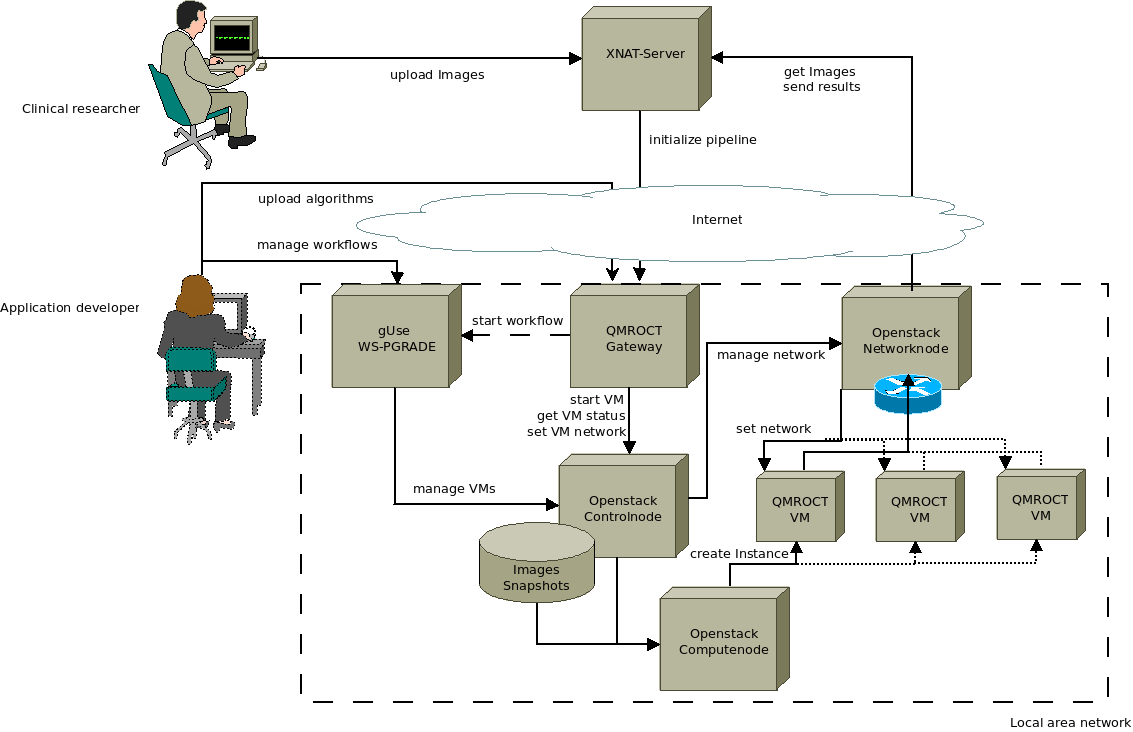
\includegraphics[width=2.0\columnwidth]{images/somno-architecture.png}
                \caption{Architecture of QM-ROCT \cite{wu14} including WS-PGRADE/gUSE}
                \label{fig:architecture}
\end{figure*}

\subsection{Configuration}\label{configuration}

The cloud plugin of the DCI bridge ships with gUSE and is activated by default.

A new configuration, as can be seen in figure~\ref{fig:cloudconfig}, is created in the web interface under \textit{Information, Resources, Cloud}.
In this case the name of the configuration is set as \textit{local cloud} and the status is \textit{enabled}. The field service and parameters specifies three important settings.
The first part is the URL referencing the EC2 interface of OpenStack and can be found in the OpenStack web interface under \textit{Access \& Security, API Access}.
The second parameter is the EC2 ID of the image or snapshot, the Virtual Machine is based on.
This EC2 ID is not the same as the ID listed in the OpenStack web interface, which is only suitable for the Nova API.
The EC2 ID can be determined by using the euca2ools command \textit{euca-describe-instances}.
The third parameters is the maximum number of VM instances managed at once.
This number should not be higher than the number of instances that can actually be handled by the given cloud resources.
gUSE will not determine the load of the cloud.

After creating the new cloud configuration the security credentials must be given under \textit{security, cloud, local cloud}.
The EC2 credentials for OpenStack can be downloaded from the OpenStack EC2 web interface under \textit{Access \& Security, API Access, Download EC2 Credentials}.
The downloaded archive contains a text file named \textit{ec2rc.sh}, which contains the necessary values.
The value of the variable \textit{EC2\_ACCESS\_KEY} maps to the user field and \textit{EC2\_SECRET\_KEY} maps to the password field of gUSE.

\begin{figure*}%[!b]
                \centering
                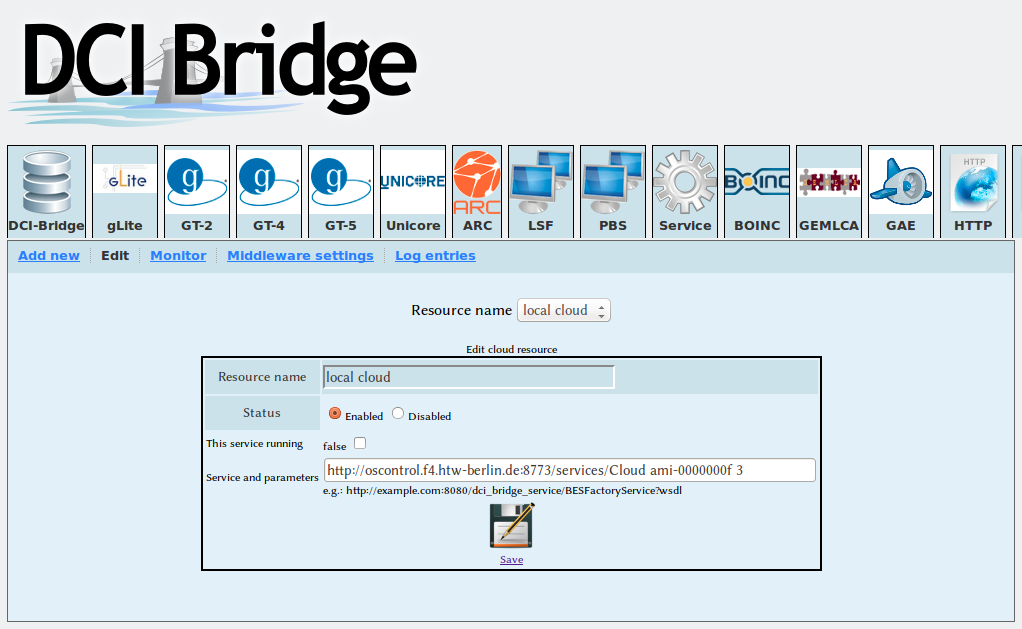
\includegraphics[width=2.0\columnwidth]{images/dci-cloud-settings.png}
                \caption{DCI cloud configuration}
                \label{fig:cloudconfig}
\end{figure*}

With the given information gUSE is able to run euca2ools commands in order to create and terminate VM instances and to determine the IP address of a running VM.
A problem that occurred with euca2ools, the EC2 interface and the cloud configuration in the private network, is the wrong assignment of public IP addresses.
The public IP address, that got assigned was not reachable inside the network and therefore not usable.
This is probably a bug with the EC2 API of OpenStack or a wrong command sent by euca2ools.
The solution to this problem were customized start and terminate scripts \cite{customscripts} which use Nova tools~\ref{euca} instead of the EC2 API.
These customized scripts replace the programs \textit{euca-run-instances} and \textit{euca-terminate-instances} in the directory \textit{/usr/bin} of the gUSE server.

\subsection{Workflows}\label{workflowimplementation}

How to create

Alternative solutions

Workflows: \cite{somnocqrs} \cite{somnocqrsdl} \cite{somnocqrsone}